\documentclass{beamer}
\usetheme[pageofpages=of,% String used between the current page and the
                         % total page count.
          bullet=circle,% Use circles instead of squares for bullets.
          titleline=true,% Show a line below the frame title.
          alternativetitlepage=true,% Use the fancy title page.
       %   titlepagelogo=logo-polito,% Logo for the first page.
       %   watermark=watermark-polito,% Watermark used in every page.
       %   watermarkheight=100px,% Height of the watermark.
       %   watermarkheightmult=4,% The watermark image is 4 times bigger
                                % than watermarkheight.
          ]{Torino}

\setbeamertemplate{footline}{
  \begin{beamercolorbox}[wd=\paperwidth,ht=1ex,dp=1ex]{footline}
    \vspace{5pt} \hspace{1em} \insertframenumber/\inserttotalframenumber
  \end{beamercolorbox}
}

\author{Brendon J. Brewer}
\title{STATS 331 -- Introduction to Bayesian Statistics}
\institute{The University of Auckland}
\date{}


\linespread{1.3}
\usepackage{minted}
\usepackage[utf8]{inputenc}
\usepackage{dsfont}
\newcommand{\given}{\,|\,}
\newcommand{\balpha}{\boldsymbol{\alpha}}
\newcommand{\bmu}{\boldsymbol{\mu}}


\begin{document}

\frame{\titlepage}

\begin{frame}
\Large

\begin{center}
Review
\end{center}
\end{frame}

\begin{frame}
\frametitle{Lecture Purpose}

We will now briefly review the course content, and I will outline my
expectations for what you should be able to do in the exam.

\end{frame}


\begin{frame}
\frametitle{Probabilities}
The mathematics of {\bf probabilities} can be used to describe two different
things: proportions, and uncertainties. Which interpretation you adopt
determines the way you end up using the maths.\pause

   \begin{columns} % Create two columns

        \column{0.5\textwidth} % Left column (50% width)
        \centering
        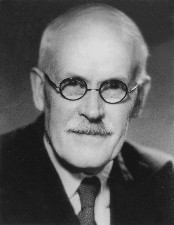
\includegraphics[width=0.5\linewidth]{images/jeffreys.jpg}

        Harold Jeffreys (Bayesian)

        \column{0.5\textwidth} % Right column (50% width)
        \centering
        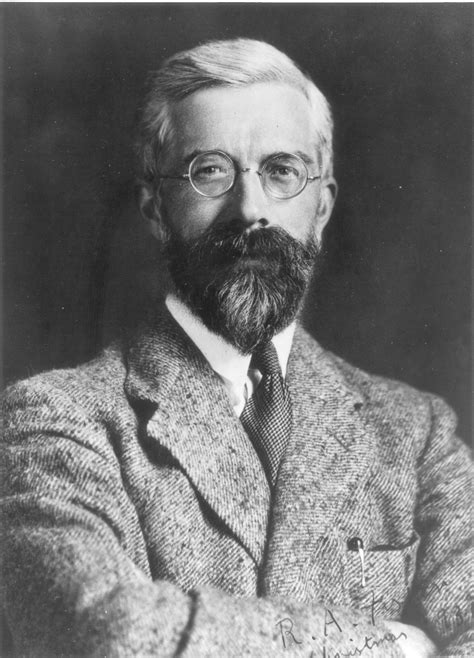
\includegraphics[width=0.5\linewidth]{images/fisher.jpg}

        R. A. Fisher (Frequentist)
     \end{columns}


\end{frame}


\begin{frame}
\frametitle{Rules of Probability}
Fundamentally, there are two rules of probability, the sum rule and the
product rule. Their most general versions are given below.

\begin{align}
P(A \vee B \given C) &= P(A \given C) + P(B \given C) - P(A, B \given C) \\
P(A, B \given C) &= P(A \given C)P(B \given A, C).
\end{align}\pause

Other rules such as Bayes' rule and the partition theorem are derived from
these.


\end{frame}


\begin{frame}
\frametitle{Sum Rule Applications}
The sum rule shows up in Bayesian statistics in a few different situations:\pause

\begin{itemize}
\item Prior and posterior probabilities of `OR' statements (a popular exam
question that is easy marks).\pause
\item Marginal likelihood calculation.\pause
\item Predictions.\pause
\item Finding marginal posterior distributions (for one parameter only)
from joint distributions (of more than one parameter).
\end{itemize}


\end{frame}


\begin{frame}
\frametitle{Product Rule Applications}
The product rule shows up in Bayesian statistics in a few different situations:\pause

\begin{itemize}
\item Bayes' rule, used for updating probabilities, comes from the product
rule.\pause
\item Joint distributions are formed using the product rule. This is how
we can construct prior distributions for more than one parameter, or
sampling distributions for more than one data value.
\end{itemize}


\end{frame}


\begin{frame}
\frametitle{Bayes' Rule}
The most important form of Bayes' rule is the one that gives you the
posterior probabilities of some mutually exclusive hypotheses $H_i$:

\begin{align}
P(H_i \given D) &= \frac{P(H_i)P(D \given H_i)}{P(D)}
\end{align} \pause
where
\begin{align}
P(D) &= \sum_i P(H_i) P(D \given H_i).
\end{align}


\end{frame}


\begin{frame}
\frametitle{Checklist for Exam}

\begin{itemize}
\item Ideally, know these rules from memory (but you can use your cheat sheet
too).\pause
\item Know how to do a Bayes Box. Part of this is being able to read the
question and to know what values go in the prior
and likelihood columns of the Bayes Box.\pause
\item Be able to write down Bayes' rule or the marginal likelihood formula
corresponding to the particular statements in a given problem.
\end{itemize}


\end{frame}


\begin{frame}
\frametitle{Parameter Estimation}
Recall that Bayes' rule can be used on a set of mutually exclusive hypotheses.
These can be statements about the value of the parameter $\theta$.\pause

\begin{itemize}
\item One hypothesis might be ``$\theta = 1$'' \pause
\item Another might be ``$\theta = 2$'' \pause
\item We might get some data like ``$x = 3$''.
\end{itemize}

\end{frame}


\begin{frame}
\frametitle{Bayes' Rule Lots of Times}
\begin{align}
P(\theta = 1 \given x = 3) &= \frac{P(\theta=1)P(x=3 \given \theta=1)}{P(x=3)}\\
P(\theta = 2 \given x = 3) &= \frac{P(\theta=2)P(x=3 \given \theta=2)}{P(x=3)}\\
&...&\\
P(\theta = 9 \given x = 3) &= \frac{P(\theta=9)P(x=3 \given \theta=9)}{P(x=3)}\\
\end{align}

\end{frame}

\begin{frame}
\frametitle{Bayes' Rule Lots of Times}
\begin{align}
\color{red}{P(\theta = 1 \given x = 3)} &= \frac{{\color{blue}P(\theta=1)}P(x=3 \given \theta=1)}{P(x=3)}\\
\color{red}{P(\theta = 2 \given x = 3)} &= \frac{{\color{blue}P(\theta=2)}P(x=3 \given \theta=2)}{P(x=3)}\\
&...&\\
\color{red}{P(\theta = 9 \given x = 3)} &= \frac{{\color{blue}P(\theta=9)}P(x=3 \given \theta=9)}{P(x=3)}\\
\end{align}

{\color{red}Posterior Distribution}
{\color{blue}Prior Distribution}

\end{frame}


\begin{frame}
\frametitle{Bayes' Rule Lots of Times}
\begin{align}
P(\theta = 1 \given x = 3) &= \frac{P(\theta=1){\color{orange}P(x=3 \given \theta=1)}}{\color{green}P(x=3)}\\
P(\theta = 2 \given x = 3) &= \frac{P(\theta=2){\color{orange}P(x=3 \given \theta=2)}}{\color{green}P(x=3)}\\
&...&\\
P(\theta = 9 \given x = 3) &= \frac{P(\theta=9){\color{orange}P(x=3 \given \theta=9)}}{\color{green}P(x=3)}\\
\end{align}

{\color{orange}Likelihood Function}
{\color{green}Marginal Likelihood (common to all $\theta$ values)}

\end{frame}

\begin{frame}
\frametitle{Bayes Box for Parameter Estimation}
Since a Bayes Box is equivalent to these repeated uses of Bayes' rule,
we can use them for parameter estimation (when there is only one unknown
parameter).

\end{frame}


\end{document}

